\documentclass[]{article}
\usepackage{lmodern}
\usepackage{amssymb,amsmath}
\usepackage{ifxetex,ifluatex}
\usepackage{fixltx2e} % provides \textsubscript
\ifnum 0\ifxetex 1\fi\ifluatex 1\fi=0 % if pdftex
  \usepackage[T1]{fontenc}
  \usepackage[utf8]{inputenc}
\else % if luatex or xelatex
  \ifxetex
    \usepackage{mathspec}
  \else
    \usepackage{fontspec}
  \fi
  \defaultfontfeatures{Ligatures=TeX,Scale=MatchLowercase}
\fi
% use upquote if available, for straight quotes in verbatim environments
\IfFileExists{upquote.sty}{\usepackage{upquote}}{}
% use microtype if available
\IfFileExists{microtype.sty}{%
\usepackage{microtype}
\UseMicrotypeSet[protrusion]{basicmath} % disable protrusion for tt fonts
}{}
\usepackage[margin=1in]{geometry}
\usepackage{hyperref}
\hypersetup{unicode=true,
            pdftitle={results},
            pdfauthor={Qi Yuchen},
            pdfborder={0 0 0},
            breaklinks=true}
\urlstyle{same}  % don't use monospace font for urls
\usepackage{color}
\usepackage{fancyvrb}
\newcommand{\VerbBar}{|}
\newcommand{\VERB}{\Verb[commandchars=\\\{\}]}
\DefineVerbatimEnvironment{Highlighting}{Verbatim}{commandchars=\\\{\}}
% Add ',fontsize=\small' for more characters per line
\usepackage{framed}
\definecolor{shadecolor}{RGB}{248,248,248}
\newenvironment{Shaded}{\begin{snugshade}}{\end{snugshade}}
\newcommand{\AlertTok}[1]{\textcolor[rgb]{0.94,0.16,0.16}{#1}}
\newcommand{\AnnotationTok}[1]{\textcolor[rgb]{0.56,0.35,0.01}{\textbf{\textit{#1}}}}
\newcommand{\AttributeTok}[1]{\textcolor[rgb]{0.77,0.63,0.00}{#1}}
\newcommand{\BaseNTok}[1]{\textcolor[rgb]{0.00,0.00,0.81}{#1}}
\newcommand{\BuiltInTok}[1]{#1}
\newcommand{\CharTok}[1]{\textcolor[rgb]{0.31,0.60,0.02}{#1}}
\newcommand{\CommentTok}[1]{\textcolor[rgb]{0.56,0.35,0.01}{\textit{#1}}}
\newcommand{\CommentVarTok}[1]{\textcolor[rgb]{0.56,0.35,0.01}{\textbf{\textit{#1}}}}
\newcommand{\ConstantTok}[1]{\textcolor[rgb]{0.00,0.00,0.00}{#1}}
\newcommand{\ControlFlowTok}[1]{\textcolor[rgb]{0.13,0.29,0.53}{\textbf{#1}}}
\newcommand{\DataTypeTok}[1]{\textcolor[rgb]{0.13,0.29,0.53}{#1}}
\newcommand{\DecValTok}[1]{\textcolor[rgb]{0.00,0.00,0.81}{#1}}
\newcommand{\DocumentationTok}[1]{\textcolor[rgb]{0.56,0.35,0.01}{\textbf{\textit{#1}}}}
\newcommand{\ErrorTok}[1]{\textcolor[rgb]{0.64,0.00,0.00}{\textbf{#1}}}
\newcommand{\ExtensionTok}[1]{#1}
\newcommand{\FloatTok}[1]{\textcolor[rgb]{0.00,0.00,0.81}{#1}}
\newcommand{\FunctionTok}[1]{\textcolor[rgb]{0.00,0.00,0.00}{#1}}
\newcommand{\ImportTok}[1]{#1}
\newcommand{\InformationTok}[1]{\textcolor[rgb]{0.56,0.35,0.01}{\textbf{\textit{#1}}}}
\newcommand{\KeywordTok}[1]{\textcolor[rgb]{0.13,0.29,0.53}{\textbf{#1}}}
\newcommand{\NormalTok}[1]{#1}
\newcommand{\OperatorTok}[1]{\textcolor[rgb]{0.81,0.36,0.00}{\textbf{#1}}}
\newcommand{\OtherTok}[1]{\textcolor[rgb]{0.56,0.35,0.01}{#1}}
\newcommand{\PreprocessorTok}[1]{\textcolor[rgb]{0.56,0.35,0.01}{\textit{#1}}}
\newcommand{\RegionMarkerTok}[1]{#1}
\newcommand{\SpecialCharTok}[1]{\textcolor[rgb]{0.00,0.00,0.00}{#1}}
\newcommand{\SpecialStringTok}[1]{\textcolor[rgb]{0.31,0.60,0.02}{#1}}
\newcommand{\StringTok}[1]{\textcolor[rgb]{0.31,0.60,0.02}{#1}}
\newcommand{\VariableTok}[1]{\textcolor[rgb]{0.00,0.00,0.00}{#1}}
\newcommand{\VerbatimStringTok}[1]{\textcolor[rgb]{0.31,0.60,0.02}{#1}}
\newcommand{\WarningTok}[1]{\textcolor[rgb]{0.56,0.35,0.01}{\textbf{\textit{#1}}}}
\usepackage{longtable,booktabs}
\usepackage{graphicx,grffile}
\makeatletter
\def\maxwidth{\ifdim\Gin@nat@width>\linewidth\linewidth\else\Gin@nat@width\fi}
\def\maxheight{\ifdim\Gin@nat@height>\textheight\textheight\else\Gin@nat@height\fi}
\makeatother
% Scale images if necessary, so that they will not overflow the page
% margins by default, and it is still possible to overwrite the defaults
% using explicit options in \includegraphics[width, height, ...]{}
\setkeys{Gin}{width=\maxwidth,height=\maxheight,keepaspectratio}
\IfFileExists{parskip.sty}{%
\usepackage{parskip}
}{% else
\setlength{\parindent}{0pt}
\setlength{\parskip}{6pt plus 2pt minus 1pt}
}
\setlength{\emergencystretch}{3em}  % prevent overfull lines
\providecommand{\tightlist}{%
  \setlength{\itemsep}{0pt}\setlength{\parskip}{0pt}}
\setcounter{secnumdepth}{0}
% Redefines (sub)paragraphs to behave more like sections
\ifx\paragraph\undefined\else
\let\oldparagraph\paragraph
\renewcommand{\paragraph}[1]{\oldparagraph{#1}\mbox{}}
\fi
\ifx\subparagraph\undefined\else
\let\oldsubparagraph\subparagraph
\renewcommand{\subparagraph}[1]{\oldsubparagraph{#1}\mbox{}}
\fi

%%% Use protect on footnotes to avoid problems with footnotes in titles
\let\rmarkdownfootnote\footnote%
\def\footnote{\protect\rmarkdownfootnote}

%%% Change title format to be more compact
\usepackage{titling}

% Create subtitle command for use in maketitle
\providecommand{\subtitle}[1]{
  \posttitle{
    \begin{center}\large#1\end{center}
    }
}

\setlength{\droptitle}{-2em}

  \title{results}
    \pretitle{\vspace{\droptitle}\centering\huge}
  \posttitle{\par}
    \author{Qi Yuchen}
    \preauthor{\centering\large\emph}
  \postauthor{\par}
      \predate{\centering\large\emph}
  \postdate{\par}
    \date{2019/12/11}


\begin{document}
\maketitle

\hypertarget{data-cleaning}{%
\section{Data cleaning}\label{data-cleaning}}

\begin{Shaded}
\begin{Highlighting}[]
\CommentTok{# import}
\NormalTok{df =}\StringTok{ }\KeywordTok{read_csv}\NormalTok{(}\StringTok{"Lawsuit.csv"}\NormalTok{) }\OperatorTok\StringTok{ }
\StringTok{  }\NormalTok{janitor}\OperatorTok{::}\KeywordTok{clean_names}\NormalTok{() }\OperatorTok\StringTok{ }
\StringTok{  }\KeywordTok{mutate}\NormalTok{(}\DataTypeTok{dept =} \KeywordTok{factor}\NormalTok{(dept, }\DataTypeTok{levels =} \KeywordTok{c}\NormalTok{(}\DecValTok{1}\OperatorTok{:}\DecValTok{6}\NormalTok{), }\DataTypeTok{labels =} \KeywordTok{c}\NormalTok{(}\StringTok{"Biochemistry/Molecular Biology"}\NormalTok{, }\StringTok{"Physiology "}\NormalTok{, }\StringTok{"Genetics"}\NormalTok{, }\StringTok{"Pediatrics"}\NormalTok{, }\StringTok{"Medicine"}\NormalTok{, }\StringTok{"Surgery"}\NormalTok{)),}
         \DataTypeTok{gender =} \KeywordTok{factor}\NormalTok{(gender, }\DataTypeTok{levels =} \KeywordTok{c}\NormalTok{(}\DecValTok{0}\NormalTok{, }\DecValTok{1}\NormalTok{), }\DataTypeTok{labels =} \KeywordTok{c}\NormalTok{(}\StringTok{"Female"}\NormalTok{,}\StringTok{"Male"}\NormalTok{)),}
         \DataTypeTok{clin =} \KeywordTok{factor}\NormalTok{(clin, }\DataTypeTok{levels =} \KeywordTok{c}\NormalTok{(}\DecValTok{1}\NormalTok{, }\DecValTok{0}\NormalTok{), }\DataTypeTok{labels =} \KeywordTok{c}\NormalTok{(}\StringTok{"Clinical"}\NormalTok{,}\StringTok{"Research"}\NormalTok{)),}
         \DataTypeTok{cert =} \KeywordTok{factor}\NormalTok{(cert, }\DataTypeTok{levels =} \KeywordTok{c}\NormalTok{(}\DecValTok{1}\NormalTok{, }\DecValTok{0}\NormalTok{), }\DataTypeTok{labels =} \KeywordTok{c}\NormalTok{(}\StringTok{"Certified"}\NormalTok{,}\StringTok{"Not certified"}\NormalTok{)),}
         \DataTypeTok{rank =} \KeywordTok{factor}\NormalTok{(rank, }\DataTypeTok{levels =} \KeywordTok{c}\NormalTok{(}\DecValTok{1}\NormalTok{, }\DecValTok{2}\NormalTok{, }\DecValTok{3}\NormalTok{), }\DataTypeTok{labels =} \KeywordTok{c}\NormalTok{(}\StringTok{"Assistant"}\NormalTok{, }\StringTok{"Associate"}\NormalTok{, }\StringTok{"Full professor"}\NormalTok{)),}
         \DataTypeTok{sal =}\NormalTok{ (sal94 }\OperatorTok{+}\StringTok{ }\NormalTok{sal95)}\OperatorTok{/}\DecValTok{2}\NormalTok{) }
\end{Highlighting}
\end{Shaded}

\begin{verbatim}
## Parsed with column specification:
## cols(
##   ID = col_double(),
##   Dept = col_double(),
##   Gender = col_double(),
##   Clin = col_double(),
##   Cert = col_double(),
##   Prate = col_double(),
##   Exper = col_double(),
##   Rank = col_double(),
##   Sal94 = col_double(),
##   Sal95 = col_double()
## )
\end{verbatim}

\begin{Shaded}
\begin{Highlighting}[]
\CommentTok{# consider log mean sal only }
\NormalTok{df_sal =}\StringTok{ }\NormalTok{df }\OperatorTok\StringTok{   }
\StringTok{  }\KeywordTok{mutate}\NormalTok{(}\DataTypeTok{log_sal =} \KeywordTok{log}\NormalTok{(sal)) }\OperatorTok\StringTok{ }
\StringTok{  }\NormalTok{dplyr}\OperatorTok{::}\KeywordTok{select}\NormalTok{(}\OperatorTok{-}\NormalTok{sal95, }\OperatorTok{-}\NormalTok{id, }\OperatorTok{-}\NormalTok{sal94, }\OperatorTok{-}\NormalTok{sal)}
\end{Highlighting}
\end{Shaded}

\hypertarget{data-exploration}{%
\section{Data exploration}\label{data-exploration}}

\hypertarget{distribution-of-the-outcome}{%
\subsection{distribution of the
outcome}\label{distribution-of-the-outcome}}

\begin{Shaded}
\begin{Highlighting}[]
\NormalTok{hist_ave <-}
\StringTok{    }\NormalTok{df }\OperatorTok\StringTok{ }
\StringTok{    }\KeywordTok{ggplot}\NormalTok{(}\KeywordTok{aes}\NormalTok{(}\DataTypeTok{x =}\NormalTok{ sal, }\DataTypeTok{y =}\NormalTok{ ..density..)) }\OperatorTok{+}
\StringTok{    }\KeywordTok{geom_histogram}\NormalTok{() }\OperatorTok{+}\StringTok{ }
\StringTok{    }\KeywordTok{labs}\NormalTok{(}\DataTypeTok{title =} \StringTok{"Distribution of Average Salary"}\NormalTok{, }\DataTypeTok{x =} \StringTok{"Average Salary"}\NormalTok{ , }\DataTypeTok{y =} \StringTok{"Density"}\NormalTok{)}

\NormalTok{qq_ave <-}
\StringTok{    }\NormalTok{df }\OperatorTok\StringTok{ }
\StringTok{    }\KeywordTok{ggplot}\NormalTok{(}\KeywordTok{aes}\NormalTok{(}\DataTypeTok{sample =}\NormalTok{ sal)) }\OperatorTok{+}\StringTok{ }
\StringTok{    }\KeywordTok{stat_qq}\NormalTok{() }\OperatorTok{+}
\StringTok{    }\KeywordTok{stat_qq_line}\NormalTok{() }\OperatorTok{+}\StringTok{ }
\StringTok{    }\KeywordTok{labs}\NormalTok{(}\DataTypeTok{title =} \StringTok{"Normal Q-Q plot of Average Salary"}\NormalTok{ , }\DataTypeTok{x =} \StringTok{"Theoretical Quantiles"}\NormalTok{, }\DataTypeTok{y =} \StringTok{"Sample Quantiles"}\NormalTok{)}

\NormalTok{hist_trans <-}
\StringTok{    }\NormalTok{df_sal }\OperatorTok\StringTok{ }
\StringTok{    }\KeywordTok{ggplot}\NormalTok{(}\KeywordTok{aes}\NormalTok{(}\DataTypeTok{x =}\NormalTok{ log_sal, }\DataTypeTok{y =}\NormalTok{ ..density..)) }\OperatorTok{+}
\StringTok{    }\KeywordTok{geom_histogram}\NormalTok{() }\OperatorTok{+}\StringTok{ }
\StringTok{    }\KeywordTok{labs}\NormalTok{(}\DataTypeTok{title =} \StringTok{"Distribution of Transformed Salary"}\NormalTok{, }\DataTypeTok{x =} \StringTok{"Transformed Salary"}\NormalTok{, }\DataTypeTok{y =} \StringTok{"Density"}\NormalTok{)}


\NormalTok{qq_trans <-}
\StringTok{    }\NormalTok{df_sal  }\OperatorTok\StringTok{ }
\StringTok{    }\KeywordTok{ggplot}\NormalTok{(}\KeywordTok{aes}\NormalTok{(}\DataTypeTok{sample =}\NormalTok{ log_sal)) }\OperatorTok{+}\StringTok{ }
\StringTok{    }\KeywordTok{stat_qq}\NormalTok{() }\OperatorTok{+}
\StringTok{    }\KeywordTok{stat_qq_line}\NormalTok{() }\OperatorTok{+}\StringTok{ }
\StringTok{    }\KeywordTok{labs}\NormalTok{(}\DataTypeTok{title =} \StringTok{"Normal Q-Q plot of Transformed Salary"}\NormalTok{ , }\DataTypeTok{x =} \StringTok{"Theoretical Quantiles"}\NormalTok{, }\DataTypeTok{y =} \StringTok{"Sample Quantiles"}\NormalTok{)}

\KeywordTok{ggarrange}\NormalTok{(hist_ave,hist_trans,qq_ave,qq_trans) }\OperatorTok\StringTok{ }
\StringTok{    }\KeywordTok{annotate_figure}\NormalTok{(}\DataTypeTok{top =} \KeywordTok{text_grob}\NormalTok{(}\StringTok{"Salary Transformation"}\NormalTok{,}\DataTypeTok{face =} \StringTok{"bold"}\NormalTok{, }\DataTypeTok{size =} \DecValTok{14}\NormalTok{))}
\end{Highlighting}
\end{Shaded}

\begin{verbatim}
## `stat_bin()` using `bins = 30`. Pick better value with `binwidth`.
## `stat_bin()` using `bins = 30`. Pick better value with `binwidth`.
\end{verbatim}

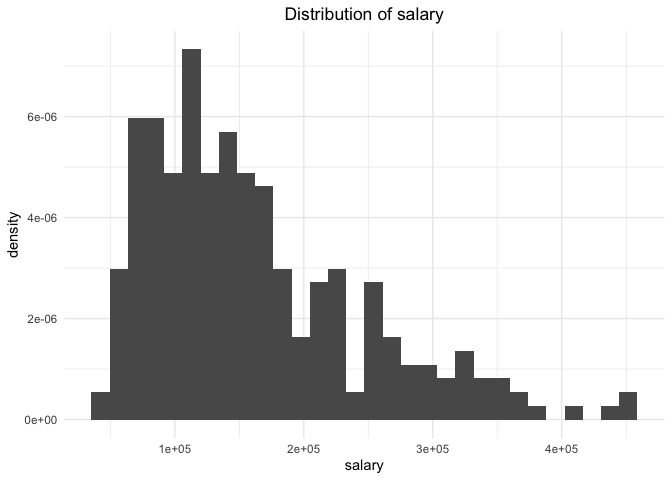
\includegraphics[width=0.9\linewidth]{results_files/figure-latex/unnamed-chunk-2-1}

From the distribution of average salary we applied log transformation to
the response variable.

\hypertarget{table1covariates-and-outcome-by-gender}{%
\subsection{table1(covariates and outcome by
gender)}\label{table1covariates-and-outcome-by-gender}}

\begin{Shaded}
\begin{Highlighting}[]
\CommentTok{# descriptive statistics for variables of interest}
\NormalTok{control_table <-}\StringTok{ }\KeywordTok{tableby.control}\NormalTok{(}
        \DataTypeTok{total =}\NormalTok{ T,}
        \DataTypeTok{test =}\NormalTok{ F,}
        \DataTypeTok{numeric.stats =} \KeywordTok{c}\NormalTok{(}\StringTok{"meansd"}\NormalTok{,}\StringTok{"medianq1q3"}\NormalTok{,}\StringTok{"range"}\NormalTok{),}
        \DataTypeTok{stats.labels =} \KeywordTok{list}\NormalTok{(}\DataTypeTok{meansd =} \StringTok{"Mean (SD)"}\NormalTok{,}
                            \DataTypeTok{medianq1q3 =} \StringTok{"Median (Q1, Q3)"}\NormalTok{,}
                            \DataTypeTok{range =} \StringTok{"Range"}\NormalTok{),}
        \DataTypeTok{digits =} \DecValTok{2}
\NormalTok{        ) }

\NormalTok{my_labels <-}\StringTok{ }\KeywordTok{list}\NormalTok{(}
  \DataTypeTok{dept =} \StringTok{"Department"}\NormalTok{,}
  \DataTypeTok{clin =} \StringTok{"Primary emphasis"}\NormalTok{,}
  \DataTypeTok{cert =} \StringTok{"Board certification"}\NormalTok{,}
  \DataTypeTok{prate =} \StringTok{"Publication rate"}\NormalTok{,}
  \DataTypeTok{exper =} \StringTok{"Experience"}\NormalTok{,}
  \DataTypeTok{rank =} \StringTok{"Rank"}\NormalTok{,}
  \DataTypeTok{log_sal =} \StringTok{"Log Salary"}
\NormalTok{)}

\NormalTok{tab1 <-}\StringTok{ }
\StringTok{    }\NormalTok{df_sal }\OperatorTok\StringTok{ }
\StringTok{    }\KeywordTok{tableby}\NormalTok{(gender }\OperatorTok{~}\StringTok{ }\NormalTok{.,}
            \DataTypeTok{data =}\NormalTok{ .,}
            \DataTypeTok{control =}\NormalTok{ control_table) }\OperatorTok\StringTok{ }
\StringTok{    }\KeywordTok{summary}\NormalTok{(}\DataTypeTok{text =} \OtherTok{TRUE}\NormalTok{,}\DataTypeTok{labelTranslations =}\NormalTok{ my_labels, }\DataTypeTok{title =} \StringTok{"Summary Statistic of Data by Gender"}\NormalTok{)}

\KeywordTok{write2pdf}\NormalTok{(tab1, }\StringTok{"table1.pdf"}\NormalTok{)}
\end{Highlighting}
\end{Shaded}

\begin{verbatim}
## 
## 
## processing file: table1.pdf.Rmd
\end{verbatim}

\begin{verbatim}
## 
  |                                                                       
  |                                                                 |   0%
  |                                                                       
  |.................................................................| 100%
##   ordinary text without R code
\end{verbatim}

\begin{verbatim}
## output file: table1.pdf.knit.md
\end{verbatim}

\begin{verbatim}
## /Applications/RStudio.app/Contents/MacOS/pandoc/pandoc +RTS -K512m -RTS table1.pdf.utf8.md --to latex --from markdown+autolink_bare_uris+ascii_identifiers+tex_math_single_backslash --output table1.tex --template /Library/Frameworks/R.framework/Versions/3.6/Resources/library/rmarkdown/rmd/latex/default-1.17.0.2.tex --highlight-style tango --pdf-engine pdflatex --variable graphics=yes --variable 'geometry:margin=1in' --variable 'compact-title:yes'
\end{verbatim}

\begin{verbatim}
## 
## Output created: table1.pdf
\end{verbatim}

\hypertarget{visualizing-the-relationship-between-response-variable-and-predictor-variables-by-gender}{%
\subsection{visualizing the relationship between response variable and
predictor variables by
gender}\label{visualizing-the-relationship-between-response-variable-and-predictor-variables-by-gender}}

categorical

\begin{Shaded}
\begin{Highlighting}[]
\NormalTok{dept_plot <-}\StringTok{ }
\StringTok{    }\NormalTok{df_sal }\OperatorTok\StringTok{ }
\StringTok{    }\KeywordTok{ggplot}\NormalTok{(}\KeywordTok{aes}\NormalTok{(}\DataTypeTok{y =}\NormalTok{ log_sal,}\DataTypeTok{x =}\NormalTok{ dept, }\DataTypeTok{fill =}\NormalTok{ gender)) }\OperatorTok{+}\StringTok{ }
\StringTok{    }\KeywordTok{geom_boxplot}\NormalTok{() }\OperatorTok{+}\StringTok{ }
\StringTok{    }\KeywordTok{labs}\NormalTok{(}\DataTypeTok{x =} \StringTok{"Department"}\NormalTok{,}\DataTypeTok{y =} \StringTok{""}\NormalTok{)}

\NormalTok{clin_plot <-}\StringTok{ }
\StringTok{    }\NormalTok{df_sal }\OperatorTok\StringTok{ }
\StringTok{    }\KeywordTok{ggplot}\NormalTok{(}\KeywordTok{aes}\NormalTok{(}\DataTypeTok{y =}\NormalTok{ log_sal,}\DataTypeTok{x =}\NormalTok{ clin, }\DataTypeTok{fill =}\NormalTok{ gender)) }\OperatorTok{+}\StringTok{ }
\StringTok{    }\KeywordTok{geom_boxplot}\NormalTok{() }\OperatorTok{+}\StringTok{ }
\StringTok{    }\KeywordTok{labs}\NormalTok{(}\DataTypeTok{x =} \StringTok{"Primary emphasis"}\NormalTok{,}\DataTypeTok{y =} \StringTok{""}\NormalTok{)}

\NormalTok{cert_plot <-}\StringTok{ }
\StringTok{    }\NormalTok{df_sal }\OperatorTok\StringTok{ }
\StringTok{    }\KeywordTok{ggplot}\NormalTok{(}\KeywordTok{aes}\NormalTok{(}\DataTypeTok{y =}\NormalTok{ log_sal,}\DataTypeTok{x =}\NormalTok{ cert, }\DataTypeTok{fill =}\NormalTok{ gender)) }\OperatorTok{+}\StringTok{ }
\StringTok{    }\KeywordTok{geom_boxplot}\NormalTok{() }\OperatorTok{+}\StringTok{ }
\StringTok{    }\KeywordTok{labs}\NormalTok{(}\DataTypeTok{x =} \StringTok{"Board certification"}\NormalTok{, }\DataTypeTok{y =} \StringTok{""}\NormalTok{)}

\NormalTok{rank_plot <-}\StringTok{ }
\StringTok{    }\NormalTok{df_sal }\OperatorTok\StringTok{ }
\StringTok{    }\KeywordTok{ggplot}\NormalTok{(}\KeywordTok{aes}\NormalTok{(}\DataTypeTok{y =}\NormalTok{ log_sal,}\DataTypeTok{x =}\NormalTok{ rank, }\DataTypeTok{fill =}\NormalTok{ gender)) }\OperatorTok{+}\StringTok{ }
\StringTok{    }\KeywordTok{geom_boxplot}\NormalTok{() }\OperatorTok{+}\StringTok{ }
\StringTok{    }\KeywordTok{labs}\NormalTok{(}\DataTypeTok{x =} \StringTok{"Rank"}\NormalTok{,}\DataTypeTok{y =} \StringTok{""}\NormalTok{)}

\NormalTok{gender_plot <-}\StringTok{ }
\StringTok{    }\NormalTok{df_sal }\OperatorTok\StringTok{ }
\StringTok{    }\KeywordTok{ggplot}\NormalTok{(}\KeywordTok{aes}\NormalTok{(}\DataTypeTok{y =}\NormalTok{ log_sal,}\DataTypeTok{x =}\NormalTok{ gender, }\DataTypeTok{fill =}\NormalTok{ gender)) }\OperatorTok{+}\StringTok{ }
\StringTok{    }\KeywordTok{geom_boxplot}\NormalTok{() }\OperatorTok{+}\StringTok{ }
\StringTok{    }\KeywordTok{labs}\NormalTok{(}\DataTypeTok{x =} \StringTok{"Gender"}\NormalTok{,}\DataTypeTok{y =} \StringTok{""}\NormalTok{)}
\end{Highlighting}
\end{Shaded}

continuous

\begin{Shaded}
\begin{Highlighting}[]
\NormalTok{prate_plot <-}
\StringTok{    }\NormalTok{df_sal }\OperatorTok\StringTok{ }
\StringTok{    }\KeywordTok{ggplot}\NormalTok{(}\KeywordTok{aes}\NormalTok{(}\DataTypeTok{y =}\NormalTok{ log_sal,}\DataTypeTok{x =}\NormalTok{ prate, }\DataTypeTok{color =}\NormalTok{ gender)) }\OperatorTok{+}\StringTok{ }
\StringTok{    }\KeywordTok{geom_point}\NormalTok{() }\OperatorTok{+}\StringTok{ }
\StringTok{    }\KeywordTok{geom_smooth}\NormalTok{(}\DataTypeTok{method =} \StringTok{"lm"}\NormalTok{,}\DataTypeTok{se =}\NormalTok{ F) }\OperatorTok{+}\StringTok{ }
\StringTok{    }\KeywordTok{labs}\NormalTok{(}\DataTypeTok{title =} \StringTok{"Salary vs Publication rate"}\NormalTok{, }\DataTypeTok{x =} \StringTok{"Publication rate"}\NormalTok{ , }\DataTypeTok{y =} \StringTok{""}\NormalTok{)}


\NormalTok{exper_plot <-}
\StringTok{    }\NormalTok{df_sal }\OperatorTok\StringTok{ }
\StringTok{    }\KeywordTok{ggplot}\NormalTok{(}\KeywordTok{aes}\NormalTok{(}\DataTypeTok{y =}\NormalTok{ log_sal,}\DataTypeTok{x =}\NormalTok{ exper, }\DataTypeTok{color =}\NormalTok{ gender)) }\OperatorTok{+}\StringTok{ }
\StringTok{    }\KeywordTok{geom_point}\NormalTok{() }\OperatorTok{+}\StringTok{ }
\StringTok{    }\KeywordTok{geom_smooth}\NormalTok{(}\DataTypeTok{method =} \StringTok{"lm"}\NormalTok{,}\DataTypeTok{se =}\NormalTok{ F) }\OperatorTok{+}
\StringTok{    }\KeywordTok{labs}\NormalTok{(}\DataTypeTok{title =} \StringTok{"Salary vs Experience"}\NormalTok{, }\DataTypeTok{x =} \StringTok{"Years since obtaining MD"}\NormalTok{, }\DataTypeTok{y =} \StringTok{""}\NormalTok{)}

\NormalTok{figure_all <-}\StringTok{ }\KeywordTok{ggarrange}\NormalTok{(dept_plot,clin_plot,cert_plot,rank_plot,gender_plot,prate_plot,exper_plot,}
                    \DataTypeTok{common.legend =}\NormalTok{ T,}\DataTypeTok{legend =} \StringTok{"bottom"}\NormalTok{)}

\CommentTok{# Annotate the figure by adding a common labels}
\KeywordTok{annotate_figure}\NormalTok{(figure_all,}
                \DataTypeTok{top =} \KeywordTok{text_grob}\NormalTok{(}\StringTok{"Salary Comparison"}\NormalTok{,}\DataTypeTok{face =} \StringTok{"bold"}\NormalTok{, }\DataTypeTok{size =} \DecValTok{14}\NormalTok{),}
                \DataTypeTok{left =} \KeywordTok{text_grob}\NormalTok{(}\StringTok{"log(salary)"}\NormalTok{,}\DataTypeTok{rot =} \DecValTok{90}\NormalTok{))}
\end{Highlighting}
\end{Shaded}

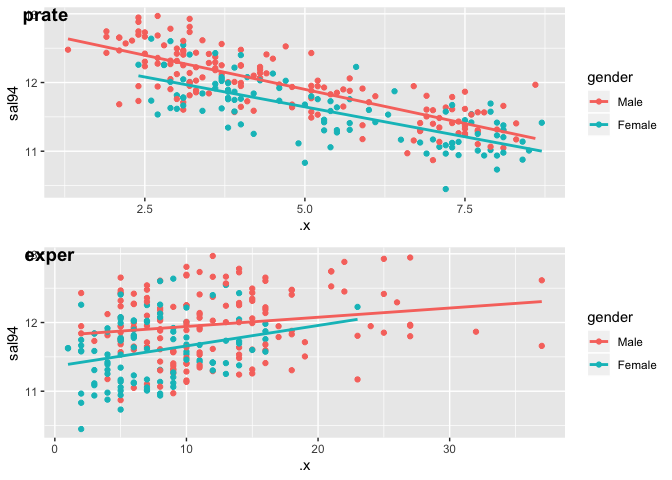
\includegraphics[width=0.9\linewidth]{results_files/figure-latex/unnamed-chunk-5-1}

We see a non-parallel(slightly) slope of \texttt{exper}, so we may
consider interaction term in our model.

\hypertarget{model}{%
\section{Model}\label{model}}

\hypertarget{main-effects}{%
\subsection{main effects}\label{main-effects}}

\hypertarget{confounders}{%
\subsubsection{Confounders}\label{confounders}}

First we consider confounders.

We check the adjusted and crude coefficients of gendermale.

\begin{Shaded}
\begin{Highlighting}[]
\NormalTok{crude <-}\StringTok{ }
\StringTok{    }\KeywordTok{lm}\NormalTok{(log_sal }\OperatorTok{~}\StringTok{ }\NormalTok{gender, }\DataTypeTok{data =}\NormalTok{ df_sal) }\OperatorTok\StringTok{ }
\StringTok{    }\NormalTok{broom}\OperatorTok{::}\KeywordTok{tidy}\NormalTok{() }\OperatorTok\StringTok{ }
\StringTok{    }\KeywordTok{filter}\NormalTok{(term }\OperatorTok{==}\StringTok{ "genderMale"}\NormalTok{) }\OperatorTok\StringTok{ }
\StringTok{    }\KeywordTok{pull}\NormalTok{(estimate)}

\NormalTok{adj <-}
\StringTok{    }\NormalTok{df_sal }\OperatorTok\StringTok{ }
\StringTok{    }\NormalTok{dplyr}\OperatorTok{::}\KeywordTok{select}\NormalTok{(dept,clin,cert,prate,exper,rank) }\OperatorTok\StringTok{ }
\StringTok{    }\KeywordTok{map}\NormalTok{(}\OperatorTok{~}\KeywordTok{lm}\NormalTok{(log_sal }\OperatorTok{~}\StringTok{ }\NormalTok{gender }\OperatorTok{+}\StringTok{ }\NormalTok{.x, }\DataTypeTok{data =}\NormalTok{ df_sal) }\OperatorTok\StringTok{ }\NormalTok{broom}\OperatorTok{::}\KeywordTok{tidy}\NormalTok{()) }\OperatorTok\StringTok{ }
\StringTok{    }\KeywordTok{map_dbl}\NormalTok{(}\OperatorTok{~}\KeywordTok{filter}\NormalTok{(.x,term }\OperatorTok{==}\StringTok{ "genderMale"}\NormalTok{) }\OperatorTok\StringTok{ }\KeywordTok{pull}\NormalTok{(estimate)) }

\NormalTok{change <-}\StringTok{ }\KeywordTok{round}\NormalTok{(}\DecValTok{100}\OperatorTok{*}\NormalTok{(crude }\OperatorTok{-}\StringTok{ }\NormalTok{adj)}\OperatorTok{/}\NormalTok{crude,}\DataTypeTok{digits =} \DecValTok{2}\NormalTok{)}
\NormalTok{change }
\end{Highlighting}
\end{Shaded}

\begin{verbatim}
##  dept  clin  cert prate exper  rank 
## 46.74 12.49 13.61 34.65 20.18  9.30
\end{verbatim}

As the magtitude of each coefficient change is around or larger than
10\%, all covariates may be confounders.Then we inlcude them all in the
model.

\hypertarget{use-vif-to-see-collinearity}{%
\subsubsection{Use VIF to see
collinearity}\label{use-vif-to-see-collinearity}}

\begin{Shaded}
\begin{Highlighting}[]
\NormalTok{full =}\StringTok{ }\KeywordTok{lm}\NormalTok{(log_sal }\OperatorTok{~}\StringTok{ }\NormalTok{., }\DataTypeTok{data =}\NormalTok{ df_sal)}

\KeywordTok{vif}\NormalTok{(full)}
\end{Highlighting}
\end{Shaded}

\begin{verbatim}
##    deptPhysiology        deptGenetics     deptPediatrics 
##           1.607184           1.629419           4.282664 
##       deptMedicine        deptSurgery         genderMale 
##           6.379551           7.215586           1.443762 
##       clinResearch  certNot certified              prate 
##           5.877635           1.329952          16.626048 
##              exper      rankAssociate rankFull professor 
##           1.884661           1.508016           2.225837
\end{verbatim}

Since prate's VIF is more than 10, we may drop it.

\begin{Shaded}
\begin{Highlighting}[]
\NormalTok{fit =}\StringTok{ }\KeywordTok{lm}\NormalTok{(log_sal }\OperatorTok{~}\NormalTok{gender}\OperatorTok{+}\NormalTok{dept}\OperatorTok{+}\NormalTok{clin}\OperatorTok{+}\NormalTok{cert}\OperatorTok{+}\NormalTok{exper}\OperatorTok{+}\NormalTok{rank, }\DataTypeTok{data =}\NormalTok{ df_sal)}

\KeywordTok{vif}\NormalTok{(fit)}
\end{Highlighting}
\end{Shaded}

\begin{verbatim}
##         genderMale    deptPhysiology        deptGenetics 
##           1.356319           1.607121           1.439383 
##     deptPediatrics       deptMedicine        deptSurgery 
##           1.894530           2.704003           2.392543 
##       clinResearch  certNot certified              exper 
##           1.659126           1.327650           1.852094 
##      rankAssociate rankFull professor 
##           1.499835           2.209568
\end{verbatim}

\begin{Shaded}
\begin{Highlighting}[]
\KeywordTok{anova}\NormalTok{(fit, full)}
\end{Highlighting}
\end{Shaded}

\begin{verbatim}
## Analysis of Variance Table
## 
## Model 1: log_sal ~ gender + dept + clin + cert + exper + rank
## Model 2: log_sal ~ dept + gender + clin + cert + prate + exper + rank
##   Res.Df    RSS Df Sum of Sq      F Pr(>F)
## 1    249 4.4506                           
## 2    248 4.4226  1  0.027919 1.5655  0.212
\end{verbatim}

Now each VIF \textless{} 5, which is good. F test also indicates no
prate.

\hypertarget{criteria}{%
\subsubsection{Criteria}\label{criteria}}

\begin{Shaded}
\begin{Highlighting}[]
\NormalTok{best_}\DecValTok{1}\NormalTok{ <-}\StringTok{ }\ControlFlowTok{function}\NormalTok{(model, ...) }
\NormalTok{\{}
\NormalTok{  subsets <-}\StringTok{ }\KeywordTok{regsubsets}\NormalTok{(}\KeywordTok{formula}\NormalTok{(model), }\KeywordTok{model.frame}\NormalTok{(model), }\DataTypeTok{method =} \StringTok{"exhaustive"}\NormalTok{, }\DataTypeTok{nvmax =} \OtherTok{NULL}\NormalTok{, }\DataTypeTok{force.in =} \StringTok{"genderMale"}\NormalTok{,  ...)}
\NormalTok{  subsets <-}\StringTok{ }\KeywordTok{with}\NormalTok{(}\KeywordTok{summary}\NormalTok{(subsets),}
                  \KeywordTok{cbind}\NormalTok{(}\DataTypeTok{p =} \KeywordTok{as.numeric}\NormalTok{(}\KeywordTok{rownames}\NormalTok{(which)), which, rss, rsq, adjr2, cp, bic))}
  
  \KeywordTok{return}\NormalTok{(subsets)}
\NormalTok{\}  }


\KeywordTok{best_1}\NormalTok{(full) }
\end{Highlighting}
\end{Shaded}

\begin{verbatim}
##     p (Intercept) genderMale deptPhysiology  deptGenetics deptPediatrics
## 2   2           1          1               0            0              0
## 3   3           1          1               0            0              0
## 4   4           1          1               0            0              0
## 5   5           1          1               0            0              0
## 6   6           1          1               0            0              0
## 7   7           1          1               1            0              0
## 8   8           1          1               1            0              0
## 9   9           1          1               1            0              0
## 10 10           1          1               1            1              0
## 11 11           1          1               1            1              1
## 12 12           1          1               1            1              1
##    deptMedicine deptSurgery clinResearch certNot certified prate exper
## 2             0           0            0                 0     1     0
## 3             0           0            0                 0     1     1
## 4             0           1            0                 0     1     1
## 5             1           1            0                 0     1     1
## 6             1           1            0                 1     1     1
## 7             1           1            0                 1     1     1
## 8             1           1            0                 1     1     1
## 9             1           1            0                 1     1     1
## 10            1           1            0                 1     1     1
## 11            1           1            1                 1     0     1
## 12            1           1            1                 1     1     1
##    rankAssociate rankFull professor       rss       rsq     adjr2
## 2              0                  0 23.703015 0.6478853 0.6451557
## 3              0                  0 16.097486 0.7608675 0.7580761
## 4              0                  0 12.931673 0.8078965 0.8048949
## 5              0                  0  8.397277 0.8752562 0.8728102
## 6              0                  0  7.073319 0.8949239 0.8924418
## 7              0                  0  6.164244 0.9084285 0.9058949
## 8              0                  1  5.469143 0.9187544 0.9161752
## 9              1                  1  4.987137 0.9259147 0.9232583
## 10             1                  1  4.724448 0.9298171 0.9270097
## 11             1                  1  4.450562 0.9338857 0.9309650
## 12             1                  1  4.422643 0.9343004 0.9311214
##            cp       bic
## 2  1074.14809 -255.7378
## 3   649.66754 -351.1644
## 4   474.14438 -402.7546
## 5   221.87785 -509.8826
## 6   149.63681 -549.0998
## 7   100.66037 -579.4396
## 8    63.68255 -605.1020
## 9    38.65405 -623.6173
## 10   25.92371 -632.1759
## 11   12.56554 -642.1984
## 12   13.00000 -638.2763
\end{verbatim}

\begin{Shaded}
\begin{Highlighting}[]
\NormalTok{subsets =}\StringTok{ }\KeywordTok{regsubsets}\NormalTok{(}\KeywordTok{formula}\NormalTok{(full), }\KeywordTok{model.frame}\NormalTok{(full), }\DataTypeTok{method =} \StringTok{"exhaustive"}\NormalTok{, }\DataTypeTok{nvmax =} \OtherTok{NULL}\NormalTok{, }\DataTypeTok{force.in =} \StringTok{"genderMale"}\NormalTok{)}

\CommentTok{# add interaction}

\NormalTok{fit_int =}\StringTok{ }\KeywordTok{lm}\NormalTok{(log_sal }\OperatorTok{~}\NormalTok{gender}\OperatorTok{+}\NormalTok{dept}\OperatorTok{+}\NormalTok{clin}\OperatorTok{+}\NormalTok{cert}\OperatorTok{+}\NormalTok{exper}\OperatorTok{+}\NormalTok{prate}\OperatorTok{+}\NormalTok{gender}\OperatorTok{*}\NormalTok{dept}\OperatorTok{+}\NormalTok{gender}\OperatorTok{*}\NormalTok{clin}\OperatorTok{+}\NormalTok{gender}\OperatorTok{*}\NormalTok{cert}\OperatorTok{+}\NormalTok{gender}\OperatorTok{*}\NormalTok{exper}\OperatorTok{+}\NormalTok{gender}\OperatorTok{*}\NormalTok{rank}\OperatorTok{+}\NormalTok{gender}\OperatorTok{*}\NormalTok{prate, }\DataTypeTok{data =}\NormalTok{ df_sal)}
\KeywordTok{best_1}\NormalTok{(fit_int)}
\end{Highlighting}
\end{Shaded}

\begin{verbatim}
##     p (Intercept) genderMale deptPhysiology  deptGenetics deptPediatrics
## 2   2           1          1               0            0              0
## 3   3           1          1               0            0              0
## 4   4           1          1               0            0              0
## 5   5           1          1               0            0              0
## 6   6           1          1               0            0              0
## 7   7           1          1               1            0              0
## 8   8           1          1               1            0              0
## 9   9           1          1               1            0              0
## 10 10           1          1               1            1              0
## 11 11           1          1               1            1              1
## 12 12           1          1               1            1              1
## 13 13           1          1               1            1              1
## 14 14           1          1               1            1              1
## 15 15           1          1               1            1              1
## 16 16           1          1               1            1              1
## 17 17           1          1               1            1              1
## 18 18           1          1               1            1              1
## 19 19           1          1               1            1              1
## 20 20           1          1               1            1              1
## 21 21           1          1               1            1              1
## 22 22           1          1               1            1              1
## 23 23           1          1               1            1              1
##    deptMedicine deptSurgery clinResearch certNot certified exper prate
## 2             0           0            0                 0     0     1
## 3             0           0            0                 0     1     1
## 4             0           1            0                 0     1     1
## 5             1           1            0                 0     1     1
## 6             1           1            0                 1     1     1
## 7             1           1            0                 1     1     1
## 8             1           1            0                 1     1     1
## 9             1           1            0                 1     1     1
## 10            1           1            0                 1     1     1
## 11            1           1            1                 1     1     0
## 12            1           1            1                 1     1     0
## 13            1           1            1                 1     1     0
## 14            1           1            1                 1     1     1
## 15            1           1            1                 1     1     1
## 16            1           1            1                 1     1     1
## 17            1           1            1                 1     1     1
## 18            1           1            1                 1     1     1
## 19            1           1            1                 1     1     1
## 20            1           1            1                 1     1     1
## 21            1           1            1                 1     1     1
## 22            1           1            1                 1     1     1
## 23            1           1            1                 1     1     1
##    rankAssociate rankFull professor genderMale:deptPhysiology 
## 2              0                  0                          0
## 3              0                  0                          0
## 4              0                  0                          0
## 5              0                  0                          0
## 6              0                  0                          0
## 7              0                  0                          0
## 8              0                  1                          0
## 9              1                  1                          0
## 10             1                  1                          0
## 11             1                  1                          0
## 12             1                  1                          0
## 13             1                  1                          0
## 14             1                  1                          0
## 15             1                  1                          0
## 16             1                  1                          1
## 17             1                  1                          1
## 18             1                  1                          1
## 19             1                  1                          1
## 20             1                  1                          1
## 21             1                  1                          1
## 22             1                  1                          1
## 23             1                  1                          1
##    genderMale:deptGenetics genderMale:deptPediatrics
## 2                        0                         0
## 3                        0                         0
## 4                        0                         0
## 5                        0                         0
## 6                        0                         0
## 7                        0                         0
## 8                        0                         0
## 9                        0                         0
## 10                       0                         0
## 11                       0                         0
## 12                       0                         0
## 13                       0                         0
## 14                       0                         0
## 15                       0                         0
## 16                       0                         0
## 17                       1                         0
## 18                       1                         0
## 19                       1                         0
## 20                       1                         1
## 21                       1                         1
## 22                       1                         1
## 23                       1                         1
##    genderMale:deptMedicine genderMale:deptSurgery genderMale:clinResearch
## 2                        0                      0                       0
## 3                        0                      0                       0
## 4                        0                      0                       0
## 5                        0                      0                       0
## 6                        0                      0                       0
## 7                        0                      0                       0
## 8                        0                      0                       0
## 9                        0                      0                       0
## 10                       0                      0                       0
## 11                       0                      0                       0
## 12                       0                      0                       0
## 13                       0                      0                       1
## 14                       0                      0                       1
## 15                       0                      0                       1
## 16                       0                      0                       1
## 17                       0                      0                       1
## 18                       0                      0                       1
## 19                       0                      0                       1
## 20                       1                      1                       0
## 21                       1                      1                       0
## 22                       1                      1                       0
## 23                       1                      1                       1
##    genderMale:certNot certified genderMale:exper genderMale:rankAssociate
## 2                             0                0                        0
## 3                             0                0                        0
## 4                             0                0                        0
## 5                             0                0                        0
## 6                             0                0                        0
## 7                             0                0                        0
## 8                             0                0                        0
## 9                             0                0                        0
## 10                            0                0                        0
## 11                            0                0                        0
## 12                            0                1                        0
## 13                            0                1                        0
## 14                            0                1                        0
## 15                            0                1                        1
## 16                            0                1                        1
## 17                            0                1                        1
## 18                            1                1                        1
## 19                            1                1                        1
## 20                            0                1                        1
## 21                            1                1                        1
## 22                            1                1                        1
## 23                            1                1                        1
##    genderMale:rankFull professor genderMale:prate       rss       rsq
## 2                              0                0 23.703015 0.6478853
## 3                              0                0 16.097486 0.7608675
## 4                              0                0 12.931673 0.8078965
## 5                              0                0  8.397277 0.8752562
## 6                              0                0  7.073319 0.8949239
## 7                              0                0  6.164244 0.9084285
## 8                              0                0  5.469143 0.9187544
## 9                              0                0  4.987137 0.9259147
## 10                             0                0  4.724448 0.9298171
## 11                             0                0  4.450562 0.9338857
## 12                             0                0  4.265977 0.9366278
## 13                             0                0  4.226133 0.9372197
## 14                             0                0  4.201395 0.9375871
## 15                             0                0  4.186764 0.9378045
## 16                             0                0  4.176169 0.9379619
## 17                             0                0  4.165282 0.9381236
## 18                             0                0  4.156955 0.9382473
## 19                             1                0  4.155045 0.9382757
## 20                             0                1  4.142562 0.9384611
## 21                             0                1  4.139394 0.9385082
## 22                             1                1  4.137467 0.9385368
## 23                             1                1  4.137269 0.9385397
##        adjr2          cp       bic
## 2  0.6451557 1102.807339 -255.7378
## 3  0.7580761  669.130965 -351.1644
## 4  0.8048949  489.780033 -402.7546
## 5  0.8728102  232.030976 -509.8826
## 6  0.8924418  158.189136 -549.0998
## 7  0.9058949  108.113542 -579.4396
## 8  0.9161752   70.295277 -605.1020
## 9  0.9232583   44.683982 -623.6173
## 10 0.9270097   31.636022 -632.1759
## 11 0.9309650   17.946702 -642.1984
## 12 0.9335614    9.372932 -647.6896
## 13 0.9339154    9.090458 -644.5743
## 14 0.9340352    9.673400 -640.5420
## 15 0.9339966   10.835275 -635.8880
## 16 0.9338938   12.228352 -630.9848
## 17 0.9337948   13.604659 -626.1016
## 18 0.9336541   15.127711 -621.0593
## 19 0.9334095   17.018269 -615.6148
## 20 0.9333329   18.303182 -610.8356
## 21 0.9331051   20.121708 -605.4707
## 22 0.9328553   22.011309 -600.0277
## 23 0.9325752   24.000000 -594.4757
\end{verbatim}

\begin{Shaded}
\begin{Highlighting}[]
\NormalTok{fit_optimal =}\StringTok{ }\KeywordTok{lm}\NormalTok{(log_sal }\OperatorTok{~}\NormalTok{gender}\OperatorTok{+}\NormalTok{dept}\OperatorTok{+}\NormalTok{clin}\OperatorTok{+}\NormalTok{cert}\OperatorTok{+}\NormalTok{exper}\OperatorTok{+}\NormalTok{gender}\OperatorTok{*}\NormalTok{clin}\OperatorTok{+}\NormalTok{gender}\OperatorTok{*}\NormalTok{exper, }\DataTypeTok{data =}\NormalTok{ df_sal)}
\KeywordTok{summary}\NormalTok{(fit_optimal)}
\end{Highlighting}
\end{Shaded}

\begin{verbatim}
## 
## Call:
## lm(formula = log_sal ~ gender + dept + clin + cert + exper + 
##     gender * clin + gender * exper, data = df_sal)
## 
## Residuals:
##      Min       1Q   Median       3Q      Max 
## -0.35192 -0.09065 -0.00500  0.08881  0.77991 
## 
## Coefficients:
##                          Estimate Std. Error t value Pr(>|t|)    
## (Intercept)             11.273377   0.045622 247.104  < 2e-16 ***
## genderMale               0.166947   0.040571   4.115 5.27e-05 ***
## deptPhysiology          -0.142009   0.031436  -4.517 9.67e-06 ***
## deptGenetics             0.212877   0.039762   5.354 1.96e-07 ***
## deptPediatrics           0.216747   0.038482   5.632 4.79e-08 ***
## deptMedicine             0.542406   0.031826  17.043  < 2e-16 ***
## deptSurgery              0.935610   0.038576  24.253  < 2e-16 ***
## clinResearch            -0.274459   0.030797  -8.912  < 2e-16 ***
## certNot certified       -0.181843   0.022805  -7.974 5.58e-14 ***
## exper                    0.040964   0.003482  11.765  < 2e-16 ***
## genderMale:clinResearch  0.127953   0.038569   3.318  0.00104 ** 
## genderMale:exper        -0.018000   0.003844  -4.683 4.65e-06 ***
## ---
## Signif. codes:  0 '***' 0.001 '**' 0.01 '*' 0.05 '.' 0.1 ' ' 1
## 
## Residual standard error: 0.1436 on 249 degrees of freedom
## Multiple R-squared:  0.9237, Adjusted R-squared:  0.9203 
## F-statistic:   274 on 11 and 249 DF,  p-value: < 2.2e-16
\end{verbatim}

So is using criteria. If force in gender, the best is without prate.
clin and exper interaction will be selected if add interaction terms.

\hypertarget{interaction-term-not-sure-whether-to-test}{%
\subsection{interaction term (not sure whether to
test)}\label{interaction-term-not-sure-whether-to-test}}

\begin{Shaded}
\begin{Highlighting}[]
\CommentTok{## general test }

\CommentTok{# no prate}
\NormalTok{fit_conf =}\StringTok{ }\KeywordTok{lm}\NormalTok{(log_sal }\OperatorTok{~}\NormalTok{gender}\OperatorTok{+}\NormalTok{dept}\OperatorTok{+}\NormalTok{clin}\OperatorTok{+}\NormalTok{cert}\OperatorTok{+}\NormalTok{exper}\OperatorTok{+}\NormalTok{rank, }\DataTypeTok{data =}\NormalTok{ df_sal)}
\KeywordTok{summary}\NormalTok{(fit_conf)}
\end{Highlighting}
\end{Shaded}

Call: lm(formula = log\_sal \textasciitilde{} gender + dept + clin +
cert + exper + rank, data = df\_sal)

Residuals: Min 1Q Median 3Q Max -0.34605 -0.07696 -0.01873 0.07596
0.90393

Coefficients: Estimate Std. Error t value
Pr(\textgreater{}\textbar{}t\textbar{})\\
(Intercept) 11.373862 0.034398 330.651 \textless{} 2e-16 \textbf{\emph{
genderMale 0.025763 0.019624 1.313 0.19\\
deptPhysiology -0.175749 0.029122 -6.035 5.73e-09 }} deptGenetics
0.185970 0.036501 5.095 6.90e-07 \textbf{\emph{ deptPediatrics 0.203345
0.035712 5.694 3.48e-08 }} deptMedicine 0.539304 0.029515 18.272
\textless{} 2e-16 \textbf{\emph{ deptSurgery 0.933820 0.035533 26.280
\textless{} 2e-16 }} clinResearch -0.208340 0.021885 -9.520 \textless{}
2e-16 \textbf{\emph{ certNot certified -0.189749 0.021244 -8.932
\textless{} 2e-16 }} exper 0.017726 0.001812 9.783 \textless{} 2e-16
\textbf{\emph{ rankAssociate 0.134663 0.023557 5.716 3.10e-08 }}
rankFull professor 0.222214 0.026249 8.466 2.22e-15 *** --- Signif.
codes: 0 `\emph{\textbf{' 0.001 '}' 0.01 '}' 0.05 `.' 0.1 ' ' 1

Residual standard error: 0.1337 on 249 degrees of freedom Multiple
R-squared: 0.9339, Adjusted R-squared: 0.931 F-statistic: 319.7 on 11
and 249 DF, p-value: \textless{} 2.2e-16

\begin{Shaded}
\begin{Highlighting}[]
\NormalTok{fit_int =}\StringTok{ }\KeywordTok{lm}\NormalTok{(log_sal }\OperatorTok{~}\NormalTok{gender}\OperatorTok{+}\NormalTok{dept}\OperatorTok{+}\NormalTok{clin}\OperatorTok{+}\NormalTok{cert}\OperatorTok{+}\NormalTok{exper}\OperatorTok{+}\NormalTok{rank}\OperatorTok{+}\NormalTok{gender}\OperatorTok{*}\NormalTok{exper, }\DataTypeTok{data =}\NormalTok{ df_sal)}
\KeywordTok{summary}\NormalTok{(fit_int)}
\end{Highlighting}
\end{Shaded}

Call: lm(formula = log\_sal \textasciitilde{} gender + dept + clin +
cert + exper + rank + gender * exper, data = df\_sal)

Residuals: Min 1Q Median 3Q Max -0.32130 -0.07860 -0.00987 0.07100
0.86910

Coefficients: Estimate Std. Error t value
Pr(\textgreater{}\textbar{}t\textbar{})\\
(Intercept) 11.293666 0.041691 270.893 \textless{} 2e-16 \textbf{\emph{
genderMale 0.128932 0.036912 3.493 0.000566 }} deptPhysiology -0.165069
0.028755 -5.741 2.75e-08 \textbf{\emph{ deptGenetics 0.189770 0.035827
5.297 2.60e-07 }} deptPediatrics 0.218603 0.035342 6.185 2.54e-09
\textbf{\emph{ deptMedicine 0.546771 0.029045 18.825 \textless{} 2e-16
}} deptSurgery 0.939830 0.034907 26.924 \textless{} 2e-16 \textbf{\emph{
clinResearch -0.208175 0.021470 -9.696 \textless{} 2e-16 }} certNot
certified -0.182166 0.020969 -8.688 5.09e-16 \textbf{\emph{ exper
0.027774 0.003545 7.834 1.38e-13 }} rankAssociate 0.118231 0.023648
5.000 1.09e-06 \textbf{\emph{ rankFull professor 0.208036 0.026112 7.967
5.90e-14 }} genderMale:exper -0.011728 0.003580 -3.276 0.001204 ** ---
Signif. codes: 0 `\emph{\textbf{' 0.001 '}' 0.01 '}' 0.05 `.' 0.1 ' ' 1

Residual standard error: 0.1312 on 248 degrees of freedom Multiple
R-squared: 0.9366, Adjusted R-squared: 0.9336 F-statistic: 305.4 on 12
and 248 DF, p-value: \textless{} 2.2e-16

\begin{Shaded}
\begin{Highlighting}[]
\KeywordTok{anova}\NormalTok{(fit_conf, fit_int)}
\end{Highlighting}
\end{Shaded}

Analysis of Variance Table

Model 1: log\_sal \textasciitilde{} gender + dept + clin + cert + exper
+ rank Model 2: log\_sal \textasciitilde{} gender + dept + clin + cert +
exper + rank + gender * exper Res.Df RSS Df Sum of Sq F
Pr(\textgreater{}F)\\
1 249 4.4506\\
2 248 4.2660 1 0.18458 10.731 0.001204 ** --- Signif. codes: 0
`\emph{\textbf{' 0.001 '}' 0.01 '}' 0.05 `.' 0.1 ' ' 1

\begin{Shaded}
\begin{Highlighting}[]
\KeywordTok{library}\NormalTok{(stargazer)}
\end{Highlighting}
\end{Shaded}

\begin{verbatim}
## 
## Please cite as:
\end{verbatim}

\begin{verbatim}
##  Hlavac, Marek (2018). stargazer: Well-Formatted Regression and Summary Statistics Tables.
\end{verbatim}

\begin{verbatim}
##  R package version 5.2.2. https://CRAN.R-project.org/package=stargazer
\end{verbatim}

\begin{Shaded}
\begin{Highlighting}[]
\KeywordTok{stargazer}\NormalTok{(fit_int, }\DataTypeTok{title =} \StringTok{"Results"}\NormalTok{, }\DataTypeTok{align =} \OtherTok{TRUE}\NormalTok{)}
\end{Highlighting}
\end{Shaded}

\% Table created by stargazer v.5.2.2 by Marek Hlavac, Harvard
University. E-mail: hlavac at fas.harvard.edu \% Date and time: 日, 12
15, 2019 - 16时43分12秒 \% Requires LaTeX packages: dcolumn

\begin{table}[!htbp] \centering 
  \caption{Results} 
  \label{} 
\begin{tabular}{@{\extracolsep{5pt}}lD{.}{.}{-3} } 
\\[-1.8ex]\hline 
\hline \\[-1.8ex] 
 & \multicolumn{1}{c}{\textit{Dependent variable:}} \\ 
\cline{2-2} 
\\[-1.8ex] & \multicolumn{1}{c}{log\_sal} \\ 
\hline \\[-1.8ex] 
 genderMale & 0.129^{***} \\ 
  & (0.037) \\ 
  & \\ 
 deptPhysiology  & -0.165^{***} \\ 
  & (0.029) \\ 
  & \\ 
 deptGenetics & 0.190^{***} \\ 
  & (0.036) \\ 
  & \\ 
 deptPediatrics & 0.219^{***} \\ 
  & (0.035) \\ 
  & \\ 
 deptMedicine & 0.547^{***} \\ 
  & (0.029) \\ 
  & \\ 
 deptSurgery & 0.940^{***} \\ 
  & (0.035) \\ 
  & \\ 
 clinResearch & -0.208^{***} \\ 
  & (0.021) \\ 
  & \\ 
 certNot certified & -0.182^{***} \\ 
  & (0.021) \\ 
  & \\ 
 exper & 0.028^{***} \\ 
  & (0.004) \\ 
  & \\ 
 rankAssociate & 0.118^{***} \\ 
  & (0.024) \\ 
  & \\ 
 rankFull professor & 0.208^{***} \\ 
  & (0.026) \\ 
  & \\ 
 genderMale:exper & -0.012^{***} \\ 
  & (0.004) \\ 
  & \\ 
 Constant & 11.294^{***} \\ 
  & (0.042) \\ 
  & \\ 
\hline \\[-1.8ex] 
Observations & \multicolumn{1}{c}{261} \\ 
R$^{2}$ & \multicolumn{1}{c}{0.937} \\ 
Adjusted R$^{2}$ & \multicolumn{1}{c}{0.934} \\ 
Residual Std. Error & \multicolumn{1}{c}{0.131 (df = 248)} \\ 
F Statistic & \multicolumn{1}{c}{305.449$^{***}$ (df = 12; 248)} \\ 
\hline 
\hline \\[-1.8ex] 
\textit{Note:}  & \multicolumn{1}{r}{$^{*}$p$<$0.1; $^{**}$p$<$0.05; $^{***}$p$<$0.01} \\ 
\end{tabular} 
\end{table}

Interaction term \(gender*exper\) is significant, thus we may conside it
in our model.

\hypertarget{stratified-regression}{%
\subsection{stratified regression}\label{stratified-regression}}

\begin{Shaded}
\begin{Highlighting}[]
\NormalTok{stratified_dept =}\StringTok{ }\NormalTok{df_sal }\OperatorTok
\StringTok{  }\KeywordTok{group_by}\NormalTok{(dept) }\OperatorTok
\StringTok{  }\KeywordTok{summarize}\NormalTok{(}
      \DataTypeTok{n =} \KeywordTok{n}\NormalTok{(),}
      \DataTypeTok{coef =}  \KeywordTok{lm}\NormalTok{(log_sal }\OperatorTok{~}\StringTok{ }\NormalTok{gender}\OperatorTok{+}\NormalTok{clin}\OperatorTok{+}\NormalTok{cert}\OperatorTok{+}\NormalTok{exper}\OperatorTok{+}\NormalTok{rank)}\OperatorTok{$}\NormalTok{coef[}\StringTok{"genderMale"}\NormalTok{],}
      \DataTypeTok{p =} \KeywordTok{summary}\NormalTok{(}\KeywordTok{lm}\NormalTok{(log_sal }\OperatorTok{~}\StringTok{ }\NormalTok{gender}\OperatorTok{+}\NormalTok{clin}\OperatorTok{+}\NormalTok{cert}\OperatorTok{+}\NormalTok{exper}\OperatorTok{+}\NormalTok{rank))}\OperatorTok{$}\NormalTok{coefficients[}\StringTok{"genderMale"}\NormalTok{,}\DecValTok{4}\NormalTok{]}
\NormalTok{            )}
\NormalTok{stratified_dept }\OperatorTok\StringTok{ }
\StringTok{    }\NormalTok{knitr}\OperatorTok{::}\KeywordTok{kable}\NormalTok{()}
\end{Highlighting}
\end{Shaded}

\begin{longtable}[]{@{}lrrr@{}}
\toprule
dept & n & coef & p\tabularnewline
\midrule
\endhead
Biochemistry/Molecular Biology & 50 & -0.0187106 &
0.6600235\tabularnewline
Physiology & 40 & -0.0052950 & 0.9224663\tabularnewline
Genetics & 21 & 0.0754572 & 0.2339215\tabularnewline
Pediatrics & 30 & 0.0115277 & 0.8453661\tabularnewline
Medicine & 80 & 0.0366927 & 0.3660339\tabularnewline
Surgery & 40 & 0.0416427 & 0.4947262\tabularnewline
\bottomrule
\end{longtable}

\begin{Shaded}
\begin{Highlighting}[]
\NormalTok{stratified_clin =}\StringTok{ }\NormalTok{df_sal }\OperatorTok
\StringTok{  }\KeywordTok{group_by}\NormalTok{(clin) }\OperatorTok
\StringTok{  }\KeywordTok{summarize}\NormalTok{(}
      \DataTypeTok{n =} \KeywordTok{n}\NormalTok{(),}
      \DataTypeTok{coef =}  \KeywordTok{lm}\NormalTok{(log_sal }\OperatorTok{~}\StringTok{ }\NormalTok{gender }\OperatorTok{+}\StringTok{ }\NormalTok{dept }\OperatorTok{+}\StringTok{ }\NormalTok{cert }\OperatorTok{+}\StringTok{ }\NormalTok{exper }\OperatorTok{+}\StringTok{ }
\StringTok{    }\NormalTok{rank)}\OperatorTok{$}\NormalTok{coef[}\StringTok{"genderMale"}\NormalTok{],}
      \DataTypeTok{p =} \KeywordTok{summary}\NormalTok{(}\KeywordTok{lm}\NormalTok{(log_sal }\OperatorTok{~}\StringTok{ }\NormalTok{gender }\OperatorTok{+}\StringTok{ }\NormalTok{dept }\OperatorTok{+}\StringTok{ }\NormalTok{cert }\OperatorTok{+}\StringTok{ }\NormalTok{exper }\OperatorTok{+}\StringTok{ }
\StringTok{    }\NormalTok{rank))}\OperatorTok{$}\NormalTok{coefficients[}\StringTok{"genderMale"}\NormalTok{,}\DecValTok{4}\NormalTok{]}
\NormalTok{            )}
\NormalTok{stratified_clin }\OperatorTok\StringTok{ }
\StringTok{    }\NormalTok{knitr}\OperatorTok{::}\KeywordTok{kable}\NormalTok{()}
\end{Highlighting}
\end{Shaded}

\begin{longtable}[]{@{}lrrr@{}}
\toprule
clin & n & coef & p\tabularnewline
\midrule
\endhead
Clinical & 160 & 0.0083165 & 0.7108663\tabularnewline
Research & 101 & 0.0465115 & 0.2948187\tabularnewline
\bottomrule
\end{longtable}

\begin{Shaded}
\begin{Highlighting}[]
\NormalTok{stratified_cert =}\StringTok{ }\NormalTok{df_sal }\OperatorTok
\StringTok{  }\KeywordTok{group_by}\NormalTok{(cert) }\OperatorTok
\StringTok{  }\KeywordTok{summarize}\NormalTok{(}
      \DataTypeTok{n =} \KeywordTok{n}\NormalTok{(),}
      \DataTypeTok{coef =}  \KeywordTok{lm}\NormalTok{(log_sal }\OperatorTok{~}\StringTok{ }\NormalTok{gender }\OperatorTok{+}\StringTok{ }\NormalTok{dept }\OperatorTok{+}\StringTok{ }\NormalTok{clin }\OperatorTok{+}\StringTok{ }\NormalTok{exper }\OperatorTok{+}\StringTok{ }
\StringTok{    }\NormalTok{rank)}\OperatorTok{$}\NormalTok{coef[}\StringTok{"genderMale"}\NormalTok{],}
      \DataTypeTok{p =} \KeywordTok{summary}\NormalTok{(}\KeywordTok{lm}\NormalTok{(log_sal }\OperatorTok{~}\StringTok{ }\NormalTok{gender }\OperatorTok{+}\StringTok{ }\NormalTok{dept }\OperatorTok{+}\StringTok{ }\NormalTok{clin }\OperatorTok{+}\StringTok{ }\NormalTok{exper }\OperatorTok{+}\StringTok{ }
\StringTok{    }\NormalTok{rank))}\OperatorTok{$}\NormalTok{coefficients[}\StringTok{"genderMale"}\NormalTok{,}\DecValTok{4}\NormalTok{]}
\NormalTok{            )}
\NormalTok{stratified_cert }\OperatorTok\StringTok{ }
\StringTok{    }\NormalTok{knitr}\OperatorTok{::}\KeywordTok{kable}\NormalTok{()}
\end{Highlighting}
\end{Shaded}

\begin{longtable}[]{@{}lrrr@{}}
\toprule
cert & n & coef & p\tabularnewline
\midrule
\endhead
Certified & 188 & 0.0126811 & 0.5584154\tabularnewline
Not certified & 73 & 0.0265111 & 0.5547041\tabularnewline
\bottomrule
\end{longtable}

\begin{Shaded}
\begin{Highlighting}[]
\NormalTok{stratified_rank =}\StringTok{ }\NormalTok{df_sal }\OperatorTok
\StringTok{  }\KeywordTok{group_by}\NormalTok{(rank) }\OperatorTok
\StringTok{  }\KeywordTok{summarize}\NormalTok{(}
      \DataTypeTok{n =} \KeywordTok{n}\NormalTok{(),}
      \DataTypeTok{coef =}  \KeywordTok{lm}\NormalTok{(log_sal }\OperatorTok{~}\StringTok{ }\NormalTok{gender }\OperatorTok{+}\StringTok{ }\NormalTok{dept }\OperatorTok{+}\StringTok{ }\NormalTok{clin }\OperatorTok{+}\StringTok{ }\NormalTok{cert }\OperatorTok{+}\StringTok{ }\NormalTok{exper)}\OperatorTok{$}\NormalTok{coef[}\StringTok{"genderMale"}\NormalTok{],}
      \DataTypeTok{p =} \KeywordTok{summary}\NormalTok{(}\KeywordTok{lm}\NormalTok{(log_sal }\OperatorTok{~}\StringTok{ }\NormalTok{gender }\OperatorTok{+}\StringTok{ }\NormalTok{dept }\OperatorTok{+}\StringTok{ }\NormalTok{clin }\OperatorTok{+}\StringTok{ }\NormalTok{cert }\OperatorTok{+}\StringTok{ }\NormalTok{exper))}\OperatorTok{$}\NormalTok{coefficients[}\StringTok{"genderMale"}\NormalTok{,}\DecValTok{4}\NormalTok{]}
\NormalTok{            )}
\NormalTok{stratified_rank }\OperatorTok\StringTok{ }
\StringTok{    }\NormalTok{knitr}\OperatorTok{::}\KeywordTok{kable}\NormalTok{()}
\end{Highlighting}
\end{Shaded}

\begin{longtable}[]{@{}lrrr@{}}
\toprule
rank & n & coef & p\tabularnewline
\midrule
\endhead
Assistant & 112 & 0.0826555 & 0.0213160\tabularnewline
Associate & 64 & -0.0132771 & 0.6702516\tabularnewline
Full professor & 85 & -0.0404129 & 0.2680458\tabularnewline
\bottomrule
\end{longtable}

\begin{Shaded}
\begin{Highlighting}[]
\NormalTok{df_exper =}\StringTok{ }\NormalTok{df_sal }\OperatorTok
\StringTok{  }\KeywordTok{mutate}\NormalTok{(}\DataTypeTok{exper_fct =} \KeywordTok{case_when}\NormalTok{(}
\NormalTok{      exper }\OperatorTok{<}\StringTok{ }\DecValTok{6} \OperatorTok{~}\StringTok{ "0"}\NormalTok{,}
\NormalTok{      exper }\OperatorTok{>=}\StringTok{ }\DecValTok{6} \OperatorTok{&}\StringTok{ }\NormalTok{exper }\OperatorTok{<}\StringTok{ }\DecValTok{9} \OperatorTok{~}\StringTok{ "1"}\NormalTok{,}
\NormalTok{      exper }\OperatorTok{>=}\StringTok{ }\DecValTok{9} \OperatorTok{&}\StringTok{ }\NormalTok{exper }\OperatorTok{<}\StringTok{ }\DecValTok{14} \OperatorTok{~}\StringTok{ "2"}\NormalTok{,}
\NormalTok{      exper }\OperatorTok{>=}\StringTok{ }\DecValTok{14} \OperatorTok{~}\StringTok{ "3"}\NormalTok{,}
      \OtherTok{TRUE} \OperatorTok{~}\StringTok{ ""}
\NormalTok{  )) }\OperatorTok\StringTok{ }
\StringTok{    }\KeywordTok{mutate}\NormalTok{(}\DataTypeTok{exper =} \KeywordTok{factor}\NormalTok{(exper_fct)) }\OperatorTok\StringTok{ }
\StringTok{    }\NormalTok{dplyr}\OperatorTok{::}\KeywordTok{select}\NormalTok{(}\OperatorTok{-}\NormalTok{exper_fct)}

\NormalTok{stratified_exper =}\StringTok{ }\NormalTok{df_exper }\OperatorTok
\StringTok{  }\KeywordTok{group_by}\NormalTok{(exper) }\OperatorTok
\StringTok{  }\KeywordTok{summarize}\NormalTok{(}
      \DataTypeTok{n =} \KeywordTok{n}\NormalTok{(),}
      \DataTypeTok{coef =}  \KeywordTok{lm}\NormalTok{(log_sal }\OperatorTok{~}\StringTok{ }\NormalTok{gender }\OperatorTok{+}\StringTok{ }\NormalTok{dept }\OperatorTok{+}\StringTok{ }\NormalTok{clin }\OperatorTok{+}\StringTok{ }\NormalTok{cert }\OperatorTok{+}\StringTok{ }\NormalTok{rank)}\OperatorTok{$}\NormalTok{coef[}\StringTok{"genderMale"}\NormalTok{],}
      \DataTypeTok{p =} \KeywordTok{summary}\NormalTok{(}\KeywordTok{lm}\NormalTok{(log_sal }\OperatorTok{~}\StringTok{ }\NormalTok{gender }\OperatorTok{+}\StringTok{ }\NormalTok{dept }\OperatorTok{+}\StringTok{ }\NormalTok{clin }\OperatorTok{+}\StringTok{ }\NormalTok{cert }\OperatorTok{+}\StringTok{ }\NormalTok{rank))}\OperatorTok{$}\NormalTok{coefficients[}\StringTok{"genderMale"}\NormalTok{,}\DecValTok{4}\NormalTok{]}
\NormalTok{            )}
\NormalTok{stratified_exper }\OperatorTok\StringTok{ }
\StringTok{    }\NormalTok{knitr}\OperatorTok{::}\KeywordTok{kable}\NormalTok{()}
\end{Highlighting}
\end{Shaded}

\begin{longtable}[]{@{}lrrr@{}}
\toprule
exper & n & coef & p\tabularnewline
\midrule
\endhead
0 & 64 & 0.1257741 & 0.0238410\tabularnewline
1 & 57 & 0.0340942 & 0.2757676\tabularnewline
2 & 74 & -0.0005508 & 0.9876466\tabularnewline
3 & 66 & -0.0034961 & 0.9439975\tabularnewline
\bottomrule
\end{longtable}

\begin{Shaded}
\begin{Highlighting}[]
\NormalTok{df_exper  }\OperatorTok
\StringTok{  }\KeywordTok{group_by}\NormalTok{(exper, rank) }\OperatorTok
\StringTok{  }\KeywordTok{summarize}\NormalTok{(}
      \DataTypeTok{n =} \KeywordTok{n}\NormalTok{())}
\end{Highlighting}
\end{Shaded}

\begin{verbatim}
## # A tibble: 11 x 3
## # Groups:   exper [4]
##    exper rank               n
##    <fct> <fct>          <int>
##  1 0     Assistant         59
##  2 0     Associate          5
##  3 1     Assistant         36
##  4 1     Associate         15
##  5 1     Full professor     6
##  6 2     Assistant         12
##  7 2     Associate         31
##  8 2     Full professor    31
##  9 3     Assistant          5
## 10 3     Associate         13
## 11 3     Full professor    48
\end{verbatim}

\hypertarget{model-diagnostics}{%
\section{Model diagnostics}\label{model-diagnostics}}

\begin{Shaded}
\begin{Highlighting}[]
\NormalTok{final_model =}\StringTok{ }\KeywordTok{lm}\NormalTok{(log_sal }\OperatorTok{~}\NormalTok{gender}\OperatorTok{+}\NormalTok{dept}\OperatorTok{+}\NormalTok{clin}\OperatorTok{+}\NormalTok{cert}\OperatorTok{+}\NormalTok{exper}\OperatorTok{+}\NormalTok{rank, }\DataTypeTok{data =}\NormalTok{ df_sal)}
\KeywordTok{par}\NormalTok{(}\DataTypeTok{mfrow =} \KeywordTok{c}\NormalTok{(}\DecValTok{2}\NormalTok{,}\DecValTok{2}\NormalTok{))}
\KeywordTok{plot}\NormalTok{(final_model)}
\end{Highlighting}
\end{Shaded}

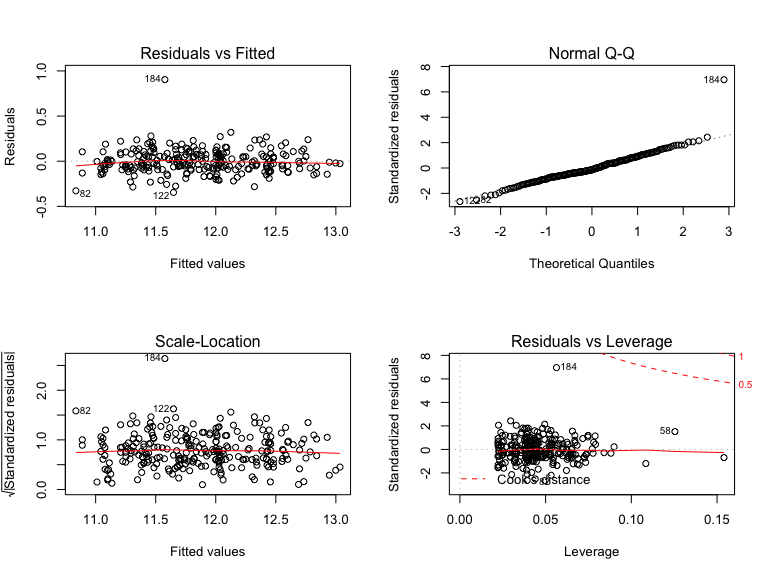
\includegraphics[width=0.9\linewidth]{results_files/figure-latex/unnamed-chunk-13-1}

\hypertarget{outliersinfluential-points}{%
\section{Outliers/influential points}\label{outliersinfluential-points}}

\begin{Shaded}
\begin{Highlighting}[]
\NormalTok{stu_res<-}\KeywordTok{rstandard}\NormalTok{(final_model)}
\NormalTok{stu_res[}\KeywordTok{abs}\NormalTok{(stu_res)}\OperatorTok{>}\FloatTok{2.5}\NormalTok{]}
\end{Highlighting}
\end{Shaded}

\begin{verbatim}
##        82       122       184 
## -2.507753 -2.640742  6.960085
\end{verbatim}

\begin{Shaded}
\begin{Highlighting}[]
\KeywordTok{influence.measures}\NormalTok{(final_model) }\OperatorTok\StringTok{ }
\StringTok{  }\KeywordTok{summary}\NormalTok{()}
\end{Highlighting}
\end{Shaded}

\begin{verbatim}
## Potentially influential observations of
##   lm(formula = log_sal ~ gender + dept + clin + cert + exper +      rank, data = df_sal) :
## 
##     dfb.1_ dfb.gndM dfb.dptPh dfb.dptG dfb.dptPd dfb.dptM dfb.dptS
## 19   0.08  -0.01     0.04      0.04     0.00      0.03     0.03   
## 82   0.01   0.07    -0.31      0.00    -0.05     -0.08    -0.11   
## 91   0.04  -0.01    -0.01     -0.08    -0.02     -0.02    -0.01   
## 109  0.00  -0.02     0.00      0.05     0.00      0.01     0.01   
## 122 -0.14   0.07     0.03      0.04    -0.27      0.08     0.06   
## 184 -0.62   0.75     0.22      0.16     0.53      1.00     0.53   
## 208  0.06  -0.19    -0.01     -0.01    -0.04      0.11    -0.02   
##     dfb.clnR dfb.crNc dfb.expr dfb.rnkA dfb.rnFp dffit   cov.r   cook.d
## 19  -0.01    -0.09    -0.26     0.05     0.17    -0.30    1.21_*  0.01 
## 82  -0.13    -0.18     0.08     0.12     0.07    -0.54    0.81_*  0.02 
## 91  -0.04     0.03    -0.04     0.02     0.01    -0.10    1.15_*  0.00 
## 109  0.02    -0.03     0.00     0.03     0.00     0.07    1.15_*  0.00 
## 122  0.11     0.02     0.02     0.10     0.05    -0.54    0.78_*  0.02 
## 184  0.94     0.84    -0.36    -0.51    -0.26     1.89_*  0.08_*  0.24 
## 208 -0.06    -0.04     0.21    -0.14    -0.18     0.43    0.81_*  0.02 
##     hat    
## 19   0.15_*
## 82   0.04  
## 91   0.09  
## 109  0.09  
## 122  0.04  
## 184  0.06  
## 208  0.03
\end{verbatim}

\begin{Shaded}
\begin{Highlighting}[]
\NormalTok{df[}\DecValTok{184}\NormalTok{,]}
\end{Highlighting}
\end{Shaded}

\begin{verbatim}
## # A tibble: 1 x 11
##      id dept   gender clin   cert    prate exper rank   sal94  sal95    sal
##   <dbl> <fct>  <fct>  <fct>  <fct>   <dbl> <dbl> <fct>  <dbl>  <dbl>  <dbl>
## 1   184 Medic~ Male   Resea~ Not ce~   5.1     2 Assi~ 250000 276163 2.63e5
\end{verbatim}

Using studentized residuals, id 184 is an outlier in Y. using leverage
values, 19 and 216 are outliers in X. Using DFFIT, 8, 184 and 216 are
influential points. Using main effects only, 184 is influential.

\begin{Shaded}
\begin{Highlighting}[]
\CommentTok{# consider the data without influential points}
\NormalTok{df_sal_noinflu =}\StringTok{ }\NormalTok{df_sal[}\OperatorTok{-}\DecValTok{184}\NormalTok{, ]}

\KeywordTok{par}\NormalTok{(}\DataTypeTok{mfrow =} \KeywordTok{c}\NormalTok{(}\DecValTok{2}\NormalTok{,}\DecValTok{2}\NormalTok{))}
\KeywordTok{plot}\NormalTok{(final_model)}
\end{Highlighting}
\end{Shaded}

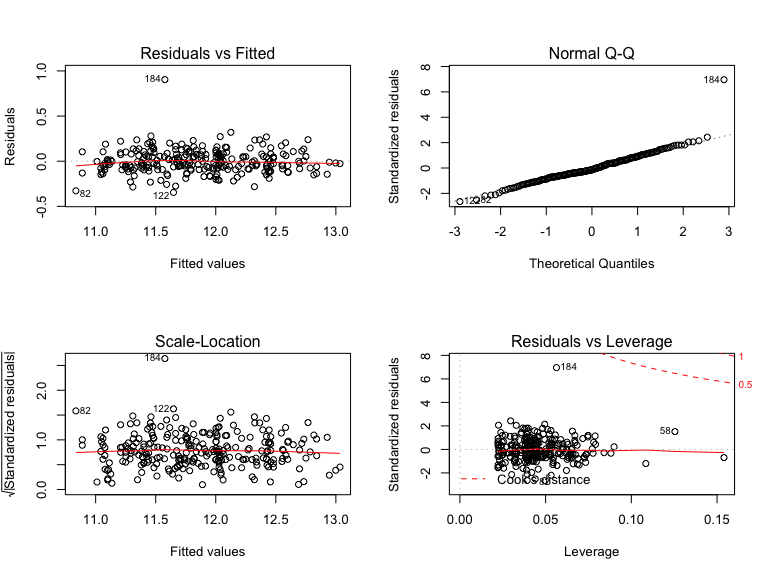
\includegraphics[width=0.9\linewidth]{results_files/figure-latex/unnamed-chunk-15-1}

\begin{Shaded}
\begin{Highlighting}[]
\NormalTok{temp =}\StringTok{ }\KeywordTok{lm}\NormalTok{(log_sal }\OperatorTok{~}\NormalTok{gender}\OperatorTok{+}\NormalTok{dept}\OperatorTok{+}\NormalTok{clin}\OperatorTok{+}\NormalTok{cert}\OperatorTok{+}\NormalTok{exper}\OperatorTok{+}\NormalTok{rank}\OperatorTok{*}\NormalTok{gender}\OperatorTok{+}\NormalTok{gender}\OperatorTok{*}\NormalTok{exper, }\DataTypeTok{data =}\NormalTok{ df_sal_noinflu)}
\KeywordTok{summary}\NormalTok{(temp)}
\end{Highlighting}
\end{Shaded}

\begin{verbatim}
## 
## Call:
## lm(formula = log_sal ~ gender + dept + clin + cert + exper + 
##     rank * gender + gender * exper, data = df_sal_noinflu)
## 
## Residuals:
##      Min       1Q   Median       3Q      Max 
## -0.32895 -0.07173 -0.01277  0.08089  0.28179 
## 
## Coefficients:
##                                Estimate Std. Error t value Pr(>|t|)    
## (Intercept)                   11.324438   0.039263 288.429  < 2e-16 ***
## genderMale                     0.100527   0.034725   2.895  0.00413 ** 
## deptPhysiology                -0.172382   0.026182  -6.584 2.77e-10 ***
## deptGenetics                   0.183611   0.032499   5.650 4.45e-08 ***
## deptPediatrics                 0.200148   0.032276   6.201 2.36e-09 ***
## deptMedicine                   0.520522   0.026654  19.529  < 2e-16 ***
## deptSurgery                    0.922849   0.031852  28.973  < 2e-16 ***
## clinResearch                  -0.225913   0.020356 -11.098  < 2e-16 ***
## certNot certified             -0.198053   0.019681 -10.063  < 2e-16 ***
## exper                          0.026606   0.003887   6.845 6.11e-11 ***
## rankAssociate                  0.138212   0.033015   4.186 3.95e-05 ***
## rankFull professor             0.213618   0.044342   4.817 2.55e-06 ***
## genderMale:rankAssociate      -0.011198   0.043888  -0.255  0.79882    
## genderMale:rankFull professor  0.002157   0.054723   0.039  0.96858    
## genderMale:exper              -0.009676   0.004265  -2.269  0.02416 *  
## ---
## Signif. codes:  0 '***' 0.001 '**' 0.01 '*' 0.05 '.' 0.1 ' ' 1
## 
## Residual standard error: 0.1188 on 245 degrees of freedom
## Multiple R-squared:  0.9483, Adjusted R-squared:  0.9454 
## F-statistic: 321.2 on 14 and 245 DF,  p-value: < 2.2e-16
\end{verbatim}

\begin{Shaded}
\begin{Highlighting}[]
\NormalTok{df_exper_noinflu =}\StringTok{ }\NormalTok{df_sal_noinflu }\OperatorTok
\StringTok{  }\KeywordTok{mutate}\NormalTok{(}\DataTypeTok{exper_fct =} \KeywordTok{case_when}\NormalTok{(}
\NormalTok{      exper }\OperatorTok{<}\StringTok{ }\DecValTok{6} \OperatorTok{~}\StringTok{ "0"}\NormalTok{,}
\NormalTok{      exper }\OperatorTok{>=}\StringTok{ }\DecValTok{6} \OperatorTok{&}\StringTok{ }\NormalTok{exper }\OperatorTok{<}\StringTok{ }\DecValTok{9} \OperatorTok{~}\StringTok{ "1"}\NormalTok{,}
\NormalTok{      exper }\OperatorTok{>=}\StringTok{ }\DecValTok{9} \OperatorTok{&}\StringTok{ }\NormalTok{exper }\OperatorTok{<}\StringTok{ }\DecValTok{14} \OperatorTok{~}\StringTok{ "2"}\NormalTok{,}
\NormalTok{      exper }\OperatorTok{>=}\StringTok{ }\DecValTok{14} \OperatorTok{~}\StringTok{ "3"}\NormalTok{,}
      \OtherTok{TRUE} \OperatorTok{~}\StringTok{ ""}
\NormalTok{  )) }\OperatorTok\StringTok{ }
\StringTok{    }\KeywordTok{mutate}\NormalTok{(}\DataTypeTok{exper =} \KeywordTok{factor}\NormalTok{(exper_fct)) }\OperatorTok\StringTok{ }
\StringTok{    }\NormalTok{dplyr}\OperatorTok{::}\KeywordTok{select}\NormalTok{(}\OperatorTok{-}\NormalTok{exper_fct)}

\NormalTok{stratified_exper_noinflu =}\StringTok{ }\NormalTok{df_exper_noinflu }\OperatorTok
\StringTok{  }\KeywordTok{group_by}\NormalTok{(exper) }\OperatorTok
\StringTok{  }\KeywordTok{summarize}\NormalTok{(}
      \DataTypeTok{n =} \KeywordTok{n}\NormalTok{(),}
      \DataTypeTok{coef =}  \KeywordTok{lm}\NormalTok{(log_sal }\OperatorTok{~}\StringTok{ }\NormalTok{gender }\OperatorTok{+}\StringTok{ }\NormalTok{dept }\OperatorTok{+}\StringTok{ }\NormalTok{clin }\OperatorTok{+}\StringTok{ }\NormalTok{cert }\OperatorTok{+}\StringTok{ }\NormalTok{rank)}\OperatorTok{$}\NormalTok{coef[}\StringTok{"genderMale"}\NormalTok{],}
      \DataTypeTok{p =} \KeywordTok{summary}\NormalTok{(}\KeywordTok{lm}\NormalTok{(log_sal }\OperatorTok{~}\StringTok{ }\NormalTok{gender }\OperatorTok{+}\StringTok{ }\NormalTok{dept }\OperatorTok{+}\StringTok{ }\NormalTok{clin }\OperatorTok{+}\StringTok{ }\NormalTok{cert }\OperatorTok{+}\StringTok{ }\NormalTok{rank))}\OperatorTok{$}\NormalTok{coefficients[}\StringTok{"genderMale"}\NormalTok{,}\DecValTok{4}\NormalTok{]}
\NormalTok{            )}
\NormalTok{stratified_exper_noinflu }\OperatorTok\StringTok{ }
\StringTok{    }\NormalTok{knitr}\OperatorTok{::}\KeywordTok{kable}\NormalTok{()}
\end{Highlighting}
\end{Shaded}

\begin{longtable}[]{@{}lrrr@{}}
\toprule
exper & n & coef & p\tabularnewline
\midrule
\endhead
0 & 63 & 0.0577437 & 0.2066119\tabularnewline
1 & 57 & 0.0340942 & 0.2757676\tabularnewline
2 & 74 & -0.0005508 & 0.9876466\tabularnewline
3 & 66 & -0.0034961 & 0.9439975\tabularnewline
\bottomrule
\end{longtable}

\begin{Shaded}
\begin{Highlighting}[]
\NormalTok{stratified_rank_noinflu =}\StringTok{ }\NormalTok{df_sal_noinflu }\OperatorTok
\StringTok{  }\KeywordTok{group_by}\NormalTok{(rank) }\OperatorTok
\StringTok{  }\KeywordTok{summarize}\NormalTok{(}
      \DataTypeTok{n =} \KeywordTok{n}\NormalTok{(),}
      \DataTypeTok{coef =}  \KeywordTok{lm}\NormalTok{(log_sal }\OperatorTok{~}\StringTok{ }\NormalTok{gender }\OperatorTok{+}\StringTok{ }\NormalTok{dept }\OperatorTok{+}\StringTok{ }\NormalTok{clin }\OperatorTok{+}\StringTok{ }\NormalTok{cert }\OperatorTok{+}\StringTok{ }\NormalTok{exper)}\OperatorTok{$}\NormalTok{coef[}\StringTok{"genderMale"}\NormalTok{],}
      \DataTypeTok{p =} \KeywordTok{summary}\NormalTok{(}\KeywordTok{lm}\NormalTok{(log_sal }\OperatorTok{~}\StringTok{ }\NormalTok{gender }\OperatorTok{+}\StringTok{ }\NormalTok{dept }\OperatorTok{+}\StringTok{ }\NormalTok{clin }\OperatorTok{+}\StringTok{ }\NormalTok{cert }\OperatorTok{+}\StringTok{ }\NormalTok{exper))}\OperatorTok{$}\NormalTok{coefficients[}\StringTok{"genderMale"}\NormalTok{,}\DecValTok{4}\NormalTok{]}
\NormalTok{            )}
\NormalTok{stratified_rank_noinflu }\OperatorTok\StringTok{ }
\StringTok{    }\NormalTok{knitr}\OperatorTok{::}\KeywordTok{kable}\NormalTok{()}
\end{Highlighting}
\end{Shaded}

\begin{longtable}[]{@{}lrrr@{}}
\toprule
rank & n & coef & p\tabularnewline
\midrule
\endhead
Assistant & 111 & 0.0390298 & 0.2009195\tabularnewline
Associate & 64 & -0.0132771 & 0.6702516\tabularnewline
Full professor & 85 & -0.0404129 & 0.2680458\tabularnewline
\bottomrule
\end{longtable}

Not significant now, -184 usinf main effects model or -216, -184, -8
using interaction model.


\end{document}
